\begin{figure}
    \centering
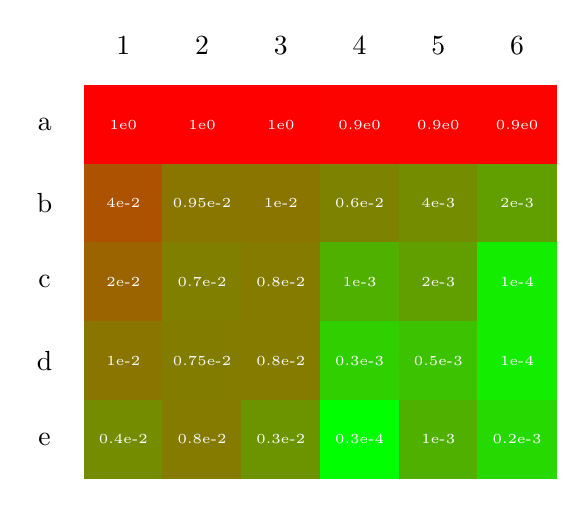
\begin{tikzpicture}
\foreach \y [count=\n] in {
{1e0, 1e0, 1e0, 0.9e0, 0.9e0, 0.9e0},
{4e-2, 0.95e-2, 1e-2, 0.6e-2, 4e-3, 2e-3},
{2e-2, 0.7e-2, 0.8e-2, 1e-3, 2e-3, 1e-4},
{1e-2, 0.75e-2, 0.8e-2, 0.3e-3, 0.5e-3, 1e-4},
{0.4e-2, 0.8e-2, 0.3e-2 ,0.3e-4, 1e-3, 0.2e-3},
} {
\node at (\n, 0) {\n};
\foreach \x [evaluate=\x as \shade using -10*ln(\x), count=\m] in \y {
\node[
fill=green!\shade!red,
minimum size=10.1mm,
text=white, font=\tiny] at (\m,-\n) {\x};
}}
\foreach \a [count=\i] in {a,b,c,d,e} {
\node at (0,-\i) {\a};
}
\end{tikzpicture}
    \caption{Caption}
    \label{fig:enter-label}
\end{figure}